\newpage
\lecture{7}{Мера с заданной функцией распределения.}

\subsection{Построение меры.}

Предположим на вещественной прямой задана монотонная непрерывная функция: $y = F(X)$ (рис. \ref{fig:lect7:1}).

\begin{figure}[!ht]
    \centering
    

\tikzset{every picture/.style={line width=0.75pt}} %set default line width to 0.75pt        

\begin{tikzpicture}[x=0.75pt,y=0.75pt,yscale=-1,xscale=1]
%uncomment if require: \path (0,300); %set diagram left start at 0, and has height of 300

%Straight Lines [id:da2460470895118685] 
\draw    (89.33,229.33) -- (517,230.33) ;
\draw [shift={(519,230.33)}, rotate = 180.13] [color={rgb, 255:red, 0; green, 0; blue, 0 }  ][line width=0.75]    (10.93,-3.29) .. controls (6.95,-1.4) and (3.31,-0.3) .. (0,0) .. controls (3.31,0.3) and (6.95,1.4) .. (10.93,3.29)   ;
%Straight Lines [id:da6618181296158356] 
\draw    (229,279.67) -- (229,93) ;
\draw [shift={(229,91)}, rotate = 450] [color={rgb, 255:red, 0; green, 0; blue, 0 }  ][line width=0.75]    (10.93,-3.29) .. controls (6.95,-1.4) and (3.31,-0.3) .. (0,0) .. controls (3.31,0.3) and (6.95,1.4) .. (10.93,3.29)   ;
%Curve Lines [id:da529846609635189] 
\draw    (115.67,223.67) .. controls (272.33,211) and (359.67,140.33) .. (457,131) ;
%Shape: Circle [id:dp22722310430147763] 
\draw  [fill={rgb, 255:red, 0; green, 0; blue, 0 }  ,fill opacity=1 ] (198.33,230.08) .. controls (198.33,229.02) and (199.19,228.17) .. (200.25,228.17) .. controls (201.31,228.17) and (202.17,229.02) .. (202.17,230.08) .. controls (202.17,231.14) and (201.31,232) .. (200.25,232) .. controls (199.19,232) and (198.33,231.14) .. (198.33,230.08) -- cycle ;
%Straight Lines [id:da17241388653795964] 
\draw  [dash pattern={on 0.84pt off 2.51pt}]  (200.33,210.17) -- (200.58,226.17) ;
%Straight Lines [id:da07476657354484773] 
\draw  [dash pattern={on 0.84pt off 2.51pt}]  (200.33,210.17) -- (229.33,210.17) ;
%Shape: Circle [id:dp3041317435730011] 
\draw  [fill={rgb, 255:red, 0; green, 0; blue, 0 }  ,fill opacity=1 ] (288,230.08) .. controls (288,229.02) and (288.86,228.17) .. (289.92,228.17) .. controls (290.98,228.17) and (291.83,229.02) .. (291.83,230.08) .. controls (291.83,231.14) and (290.98,232) .. (289.92,232) .. controls (288.86,232) and (288,231.14) .. (288,230.08) -- cycle ;
%Shape: Circle [id:dp8195691931597031] 
\draw  [fill={rgb, 255:red, 0; green, 0; blue, 0 }  ,fill opacity=1 ] (227.42,210.17) .. controls (227.42,209.11) and (228.27,208.25) .. (229.33,208.25) .. controls (230.39,208.25) and (231.25,209.11) .. (231.25,210.17) .. controls (231.25,211.23) and (230.39,212.08) .. (229.33,212.08) .. controls (228.27,212.08) and (227.42,211.23) .. (227.42,210.17) -- cycle ;
%Shape: Circle [id:dp12654824975357126] 
\draw  [fill={rgb, 255:red, 0; green, 0; blue, 0 }  ,fill opacity=1 ] (198.42,210.17) .. controls (198.42,209.11) and (199.27,208.25) .. (200.33,208.25) .. controls (201.39,208.25) and (202.25,209.11) .. (202.25,210.17) .. controls (202.25,211.23) and (201.39,212.08) .. (200.33,212.08) .. controls (199.27,212.08) and (198.42,211.23) .. (198.42,210.17) -- cycle ;
%Straight Lines [id:da28432733736513427] 
\draw  [dash pattern={on 0.84pt off 2.51pt}]  (289.67,182.83) -- (289.92,228.17) ;
%Straight Lines [id:da33803451500747306] 
\draw  [dash pattern={on 0.84pt off 2.51pt}]  (289.67,182.83) -- (228.67,182.83) ;
%Shape: Circle [id:dp8389613341648401] 
\draw  [fill={rgb, 255:red, 0; green, 0; blue, 0 }  ,fill opacity=1 ] (226.75,182.83) .. controls (226.75,181.77) and (227.61,180.92) .. (228.67,180.92) .. controls (229.73,180.92) and (230.58,181.77) .. (230.58,182.83) .. controls (230.58,183.89) and (229.73,184.75) .. (228.67,184.75) .. controls (227.61,184.75) and (226.75,183.89) .. (226.75,182.83) -- cycle ;
%Shape: Circle [id:dp1904668362422397] 
\draw  [fill={rgb, 255:red, 0; green, 0; blue, 0 }  ,fill opacity=1 ] (287.75,182.83) .. controls (287.75,181.77) and (288.61,180.92) .. (289.67,180.92) .. controls (290.73,180.92) and (291.58,181.77) .. (291.58,182.83) .. controls (291.58,183.89) and (290.73,184.75) .. (289.67,184.75) .. controls (288.61,184.75) and (287.75,183.89) .. (287.75,182.83) -- cycle ;

% Text Node
\draw (195.33,233.33) node [anchor=north west][inner sep=0.75pt]   [align=left] {$\displaystyle a$};
% Text Node
\draw (284,232) node [anchor=north west][inner sep=0.75pt]   [align=left] {$\displaystyle b$};
% Text Node
\draw (230,231.33) node [anchor=north west][inner sep=0.75pt]   [align=left] {$\displaystyle O$};
% Text Node
\draw (237,86) node [anchor=north west][inner sep=0.75pt]   [align=left] {$\displaystyle y$};
% Text Node
\draw (506.33,238) node [anchor=north west][inner sep=0.75pt]   [align=left] {$\displaystyle x$};
% Text Node
\draw (386.67,108.67) node [anchor=north west][inner sep=0.75pt]   [align=left] {$\displaystyle y=F( x)$};
% Text Node
\draw (231.67,204) node [anchor=north west][inner sep=0.75pt]  [font=\scriptsize] [align=left] {$\displaystyle F( a)$};
% Text Node
\draw (202.67,175.67) node [anchor=north west][inner sep=0.75pt]  [font=\scriptsize] [align=left] {$\displaystyle F( b)$};


\end{tikzpicture}

    \caption{Функция распределения.}
    \label{fig:lect7:1}
\end{figure}

Наша \textbf{цель}: построить
$\sigma$"=аддитивную меру $\mu$ так, что
\begin{equation}
    \mu([a,\, b])=F(b) - F(a).
    \label{eq:lect7:1}
\end{equation}

Построим даже более общую конструкцию, ослабив условие \eqref{eq:lect7:1}. Пусть $F:\: \R\rightarrow\R$ нестрого возрастает. Построим $\mu$ так, что
\[
    \mu\left((a,\,b)\right)=F(b-0)-F(a+0),
\]
где $F(b-0)=\lim\limits_{x\rightarrow b-0} F(x),\ F(a+0)=\lim\limits_{x\rightarrow a+0} F(x)$.

Пусть \[S = \{I\subset\R \ \mid\ I\text{~--- конечный промежуток, такой что } \sup I,\, \inf I\notin D\},\]
где $D$~--- множество всех точек разрыва функции $F$.
Вспомним из матанализа, что для любой монотонной функции множество ее точек разрыва не более чем счётно, более того все разрывы имеют 1 род.
Теперь определим функцию на семействе $S$: $\lambda(I)=F(\sup I)-F(\inf I)$. Исследуем свойства функции $\lambda$.
Заметим, что $S$~--- полукольцо, то есть $\lambda$~--- функция, заданная на полукольце. Более того можно заметить, что $\lambda$~---
$\sigma$"=аддитивная (доказательство строится по аналогии с клеточной мерой).

Рассмотрим $\lambda^*:\ \CP(\R)\rightarrow[0,\, +\infty]$ вида
\[
    \lambda^*(A)=\inf\left\{\sum_{n=1}^{\infty}\lambda(I_n)\ \middle|\ I_n\in S,\, A\subset \bigcup_{n=1}^{\infty}I_n\right\}.
\]
Можно заметить, что данное продолжение аналогично внешней мере Лебега.

\begin{remark}
    Если $F(x)=x\ \forall x\in\R$, то $\lambda^*$~--- в точности внешняя мера Лебега.
\end{remark}

Можно показать, что $\lambda^*$~--- внешняя мера. То есть можно проверить, что
\begin{enumerate}[label=\arabic*\degree]
    \item $\lambda^*(\varnothing)=0$;
    \item $A\subset B\Rightarrow \lambda^*(A)\leqslant\lambda^*(B)$;
    \item $\lambda^*\left(\bigcup\limits_{n=1}^{\infty}A_n\right)\leqslant \sum\limits_{n=1}^{\infty}\lambda^*(A_n)$.
\end{enumerate}

Далее рассмотрим семейство аддитивных относительно $\lambda^*$ множеств:
\[
    \CA_{\lambda^*}=\{A\subset\R\ \mid\ \forall T\subset \R:\ \lambda^*(T)=\lambda^*(T\cap A)+\lambda^*(T\setminus A)\}.
\]
По теореме Каратеодори имеем $\CA_{\lambda^*}$~--- $\sigma$"=алгебра. И $\lambda^*:\ \CA_{\lambda^*}\rightarrow[0,\,+\infty]$~--- $\sigma$"=аддитивна.
\begin{claim}
    $S\subset \CA_{\lambda^*}$.

    \begin{proof}
        Пусть $A\in S$. Докажем, что $\lambda^*(T)\geqslant\lambda^*(T\cap A)+\lambda^*(T\setminus A)$ (неравенство в обратную сторону выполнено, так как
        $\lambda^*$~--- $\sigma$"=субаддитивна).

        Пусть $T\subset\bigcup\limits_{n=1}^{\infty}A_n$, где $A_n\in S$. Тогда
        \[
            T\cap A\subset \bigcup\limits_{n=1}^{\infty}A_n\cap A,\quad T\setminus A\subset \bigcup\limits_{n=1}^{\infty}A_n\setminus A.
        \]
        Далее, так как имеем одномерный случай, то понятно, что $A_n\setminus A=B_n\sqcup C_n$, где $B_n,\, C_n\in S$ (если из интервала выкинуть интервал, получим не более двух
        интервалов). Тогда
        \[
            T\setminus A\subset \bigcup\limits_{n=1}^{\infty}A_n\setminus A=\bigcup_{n=1}^{\infty} B_n\sqcup C_n.
        \]
        Тогда имеем неравенства:
        \begin{align*}
             & \lambda^*(T\cap A)\leqslant\sum_{n=1}^{\infty}\lambda(A_n\cap A)                           \\
             & \lambda^*(T\setminus A)\leqslant\sum_{n=1}^{\infty}\left(\lambda(B_n)+\lambda(C_n)\right).
        \end{align*}
        Сложим неравенства и получим:
        \[
            \lambda^*(T\cap A)+\lambda^*(T\setminus A)\leqslant \sum_{n=1}^{\infty}\biggl[\underbrace{\lambda(A_n\cap A)+\lambda(B_n)+\lambda(C_n)}_{
            \substack{=\lambda(A_n)\text{ в силу конечной адд-ти $\lambda$,} \\ \text{т. к. } A_n=(A_n\cap A)\sqcup B_n\sqcup C_n}}\biggr].
        \]
        То есть имеем,
        \[
            \lambda^*(T\cap A)+\lambda^*(T\setminus A)\leqslant \sum_{n=1}^{\infty}\lambda (A_n)\text{, если } T\subset \bigcup_{n=1}^{\infty}A_n \text{ и }
            A_n\in S.
        \]
        Поскольку, $\lambda^*(T)=\inf \sum\limits_{n=1}^{\infty}\lambda (A_n)$, то окончательно получаем
        \[
            \lambda^*(T\cap A)+\lambda^*(T\setminus A)\leqslant\lambda^*(T).
        \]

    \end{proof}
\end{claim}

Итак,
\[
    \begin{cases}
        S\subset \CA_{\lambda^*} \\
        \CA_{\lambda^*}\text{~--- $\sigma$"=алгебра.}
    \end{cases}\biggm|\Rightarrow \sigma(S)\subset\CA_{\lambda^*}.
\]

\begin{claim}
    $\sigma(S)=\CB(\R)$.
\end{claim}

\begin{claim}
    $\forall A\in S$ имеем $\lambda^*(A)=\lambda(A)$, то есть $\lambda^*$~--- продолжение $\lambda$.

    \begin{proof}

        В самом деле, $\lambda^*(A)\leqslant\lambda(A)$~--- по определению.
        Теперь если $A\subset \bigcup\limits_{n=1}^{\infty}\Rightarrow A=\bigcup\limits_{n=1}^{\infty}A_n\cap A$. Так как $\lambda$~--- $\sigma$"=субаддитивна, то
        \[
            \lambda(A)\leqslant\sum_{n=1}^{\infty}\lambda(A_n\cap A)\leqslant\sum_{n=1}^{\infty}\lambda(A_n)\Rightarrow\lambda^*(A)\geqslant\lambda(A).
        \]

    \end{proof}
\end{claim}

Итак, $\mu(A) = \lambda^*(A)$, $A\in\CA_{\lambda^*}$~--- искомая функция.

\begin{claim}
    Если $\CE$~--- кольцо и $\mu:\ \CE\rightarrow[0,\,+\infty]$~--- конечно-аддитивна, то
    \[
        \mu\text{~---$\sigma$"=аддитивна}\Longleftrightarrow \mu\left(\bigcup_{n=1}^{\infty}A_n\right)=\lim_{N\to\infty}\mu\left(\bigcup_{n=1}^{N}A_n\right)
        \quad \forall \{A_n\}_{n=1}^{\infty}\subset\CE\text{, т. ч. } \bigcup_{n=1}^{\infty}A_n\in\CE.
    \]

    \begin{proof}

        \circled{$\Leftarrow$} Докажем $\sigma$"=аддитивность:
        \[
            \mu\left(\bigsqcup_{n=1}^{\infty}A_n\right)=\lim_{N\to\infty}\mu\left(\bigsqcup_{n=1}^N A_n\right)=[\text{в силу кон.-адд-ти}]=
            \lim_{N\to\infty}\sum_{n=1}^N\mu\left(A_n\right)=\sum_{n=1}^N\mu(A_n).
        \]

        \circled{$\Rightarrow$} Пусть $\mu$~--- $\sigma$"=аддитивна. Рассмотрим $B_n=A_n\setminus\bigcap\limits_{k=1}^{n-1}A_k$, причем $B_1=A_1$.
        Очевидно, что $B_i\cap B_j=\varnothing,\, i\neq j$, $\bigsqcup\limits_{k=1}^{\infty}B_k=\bigcup\limits_{k=1}^{\infty}A_k$.
        Тогда
        \begin{align*}
            \mu\left(\bigcup_{n=1}^{\infty}A_n\right)=\mu\left(\bigsqcup_{n=1}^{\infty}B_n\right)=\sum_{n=1}^{\infty}\mu(B_n) & =\lim_{N\to\infty}\sum_{n=1}^N\mu(B_n)=
            \lim_{N\to\infty}\mu\left(\bigsqcup_{n=1}^N B_n\right)                                                                                                                                       \\
                                                                                                                              & =\lim_{N\to\infty}\mu\left(\bigcup_{n=1}^N A_n\right),\quad\text{т. к. }
            \bigsqcup\limits_{n=1}^{N}B_n=\bigcup\limits_{n=1}^{N}A_n
        \end{align*}

    \end{proof}
\end{claim}

Проверим, что $\mu((a,\,b))=F(b-0)-F(a+0)$. Рассмотрим $\{a_n\}$~--- невозрастает и $\{b_n\}$~--- неубывает такие, что $a_n\to a$ (справа), $b_n\to b$ (слева) и $a_n,\, b_n\notin D$.
Тогда
\[
    \mu((a,\, b))=\lim_{n\to\infty}\underbrace{\mu((a_n,\, b_n))}_{=\lambda((a_n,\,b_n))}=\lim_{n\to\infty}(F(b_n)-F(a_n)),
\]
так как в силу монотонности $a_n,\, b_n$ имеем $\bigcup\limits_{n=1}^{N}(a_n,\, b_n)=(a_N,\, b_N)$.

\subsection{Функция Кантора.}

Опишем построение функции Кантора. Разделим отрезок $[0,\, 1]$ на три равных, и посередине положим значение функции равной $1/2$.
На левом отрезке проделаем то же самое, но середину положим уже за $1/4$, а на правом $3/4$. И так далее. Для лучшего пониманию смотри рисунок \ref{fig:kantor}.
Дополнительно считаем, что на $[1,\,+\infty)$ функция равна 1 и на $(-\infty,\, 0]$ функция равна 0.

\begin{figure}[!ht]
    \centering
    

\tikzset{every picture/.style={line width=0.75pt}} %set default line width to 0.75pt        

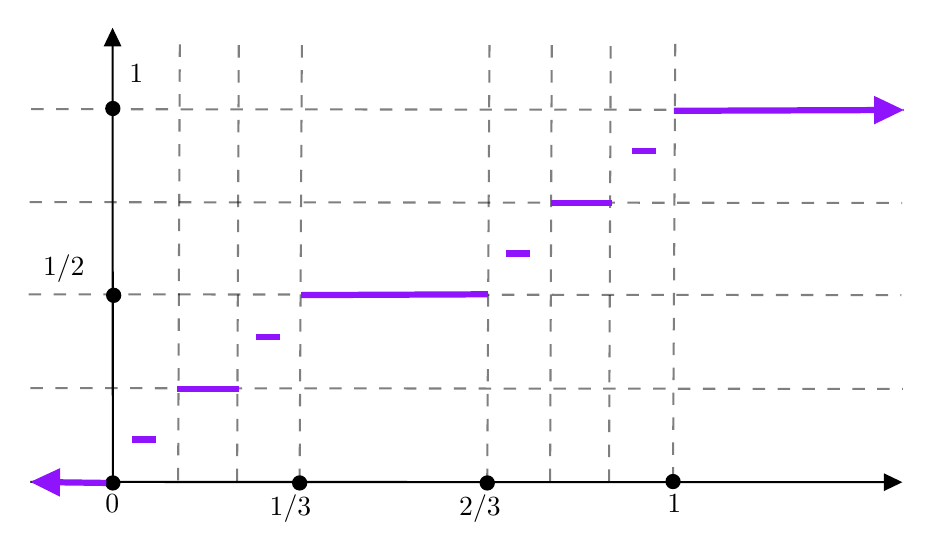
\begin{tikzpicture}[x=0.75pt,y=0.75pt,yscale=-1,xscale=1]
%uncomment if require: \path (0,300); %set diagram left start at 0, and has height of 300

%Straight Lines [id:da28165983997622934] 
\draw    (50.2,250.2) -- (467.33,250.33) ;
\draw [shift={(470.33,250.33)}, rotate = 180.02] [fill={rgb, 255:red, 0; green, 0; blue, 0 }  ][line width=0.08]  [draw opacity=0] (8.93,-4.29) -- (0,0) -- (8.93,4.29) -- cycle    ;
%Flowchart: Connector [id:dp749884860381586] 
\draw  [fill={rgb, 255:red, 0; green, 0; blue, 0 }  ,fill opacity=1 ] (86.76,250.69) .. controls (86.76,248.94) and (88.18,247.52) .. (89.93,247.52) .. controls (91.68,247.52) and (93.1,248.94) .. (93.1,250.69) .. controls (93.1,252.44) and (91.68,253.86) .. (89.93,253.86) .. controls (88.18,253.86) and (86.76,252.44) .. (86.76,250.69) -- cycle ;
%Flowchart: Connector [id:dp4945414713497278] 
\draw  [fill={rgb, 255:red, 0; green, 0; blue, 0 }  ,fill opacity=1 ] (356.67,250.02) .. controls (356.67,248.27) and (358.08,246.86) .. (359.83,246.86) .. controls (361.58,246.86) and (363,248.27) .. (363,250.02) .. controls (363,251.77) and (361.58,253.19) .. (359.83,253.19) .. controls (358.08,253.19) and (356.67,251.77) .. (356.67,250.02) -- cycle ;
%Flowchart: Connector [id:dp22339919899350247] 
\draw  [fill={rgb, 255:red, 0; green, 0; blue, 0 }  ,fill opacity=1 ] (176.76,250.69) .. controls (176.76,248.94) and (178.18,247.52) .. (179.93,247.52) .. controls (181.68,247.52) and (183.1,248.94) .. (183.1,250.69) .. controls (183.1,252.44) and (181.68,253.86) .. (179.93,253.86) .. controls (178.18,253.86) and (176.76,252.44) .. (176.76,250.69) -- cycle ;
%Flowchart: Connector [id:dp8699143961304234] 
\draw  [fill={rgb, 255:red, 0; green, 0; blue, 0 }  ,fill opacity=1 ] (267.16,250.69) .. controls (267.16,248.94) and (268.58,247.52) .. (270.33,247.52) .. controls (272.08,247.52) and (273.5,248.94) .. (273.5,250.69) .. controls (273.5,252.44) and (272.08,253.86) .. (270.33,253.86) .. controls (268.58,253.86) and (267.16,252.44) .. (267.16,250.69) -- cycle ;
%Straight Lines [id:da6785490283546702] 
\draw    (89.93,247.52) -- (89.8,34.4) ;
\draw [shift={(89.8,31.4)}, rotate = 449.97] [fill={rgb, 255:red, 0; green, 0; blue, 0 }  ][line width=0.08]  [draw opacity=0] (8.93,-4.29) -- (0,0) -- (8.93,4.29) -- cycle    ;
%Flowchart: Connector [id:dp6017519916806864] 
\draw  [fill={rgb, 255:red, 0; green, 0; blue, 0 }  ,fill opacity=1 ] (86.76,70.29) .. controls (86.76,68.54) and (88.18,67.12) .. (89.93,67.12) .. controls (91.68,67.12) and (93.1,68.54) .. (93.1,70.29) .. controls (93.1,72.04) and (91.68,73.46) .. (89.93,73.46) .. controls (88.18,73.46) and (86.76,72.04) .. (86.76,70.29) -- cycle ;
%Straight Lines [id:da7794727694597656] 
\draw [color={rgb, 255:red, 0; green, 0; blue, 0 }  ,draw opacity=0.5 ] [dash pattern={on 4.5pt off 4.5pt}]  (50.6,70.6) -- (471,71) ;
%Flowchart: Connector [id:dp9275474146310922] 
\draw  [fill={rgb, 255:red, 0; green, 0; blue, 0 }  ,fill opacity=1 ] (87.16,160.29) .. controls (87.16,158.54) and (88.58,157.12) .. (90.33,157.12) .. controls (92.08,157.12) and (93.5,158.54) .. (93.5,160.29) .. controls (93.5,162.04) and (92.08,163.46) .. (90.33,163.46) .. controls (88.58,163.46) and (87.16,162.04) .. (87.16,160.29) -- cycle ;
%Straight Lines [id:da11073911854340657] 
\draw [color={rgb, 255:red, 0; green, 0; blue, 0 }  ,draw opacity=0.5 ] [dash pattern={on 4.5pt off 4.5pt}]  (49.4,159.8) -- (469.8,160.2) ;
%Straight Lines [id:da18609205034594312] 
\draw [color={rgb, 255:red, 0; green, 0; blue, 0 }  ,draw opacity=0.5 ] [dash pattern={on 4.5pt off 4.5pt}]  (181,39.8) -- (179.93,247.52) ;
%Straight Lines [id:da06966607544396752] 
\draw [color={rgb, 255:red, 0; green, 0; blue, 0 }  ,draw opacity=0.5 ] [dash pattern={on 4.5pt off 4.5pt}]  (271.4,39.8) -- (270.33,247.52) ;
%Straight Lines [id:da20245772431088271] 
\draw [color={rgb, 255:red, 0; green, 0; blue, 0 }  ,draw opacity=0.5 ] [dash pattern={on 4.5pt off 4.5pt}]  (360.9,39.13) -- (359.83,246.86) ;
%Straight Lines [id:da606177580681843] 
\draw [color={rgb, 255:red, 144; green, 19; blue, 254 }  ,draw opacity=1 ][line width=2.25]    (180.6,160.2) -- (270.6,159.8) ;
%Straight Lines [id:da6190276976837994] 
\draw [color={rgb, 255:red, 0; green, 0; blue, 0 }  ,draw opacity=0.5 ] [dash pattern={on 4.5pt off 4.5pt}]  (301.4,39.8) -- (300.6,249.8) ;
%Straight Lines [id:da01438202404019795] 
\draw [color={rgb, 255:red, 0; green, 0; blue, 0 }  ,draw opacity=0.5 ] [dash pattern={on 4.5pt off 4.5pt}]  (329.8,40.2) -- (329,250.2) ;
%Straight Lines [id:da48628391564380014] 
\draw [color={rgb, 255:red, 0; green, 0; blue, 0 }  ,draw opacity=0.5 ] [dash pattern={on 4.5pt off 4.5pt}]  (122.2,39.4) -- (121.4,249.4) ;
%Straight Lines [id:da39031694026462715] 
\draw [color={rgb, 255:red, 0; green, 0; blue, 0 }  ,draw opacity=0.5 ] [dash pattern={on 4.5pt off 4.5pt}]  (150.6,39.8) -- (149.8,249.8) ;
%Straight Lines [id:da09573892223203795] 
\draw [color={rgb, 255:red, 0; green, 0; blue, 0 }  ,draw opacity=0.5 ] [dash pattern={on 4.5pt off 4.5pt}]  (50.2,205) -- (470.6,205.4) ;
%Straight Lines [id:da06969893090873747] 
\draw [color={rgb, 255:red, 0; green, 0; blue, 0 }  ,draw opacity=0.5 ] [dash pattern={on 4.5pt off 4.5pt}]  (49.8,115.4) -- (470.2,115.8) ;
%Straight Lines [id:da7110895807715119] 
\draw [color={rgb, 255:red, 144; green, 19; blue, 254 }  ,draw opacity=1 ][line width=2.25]    (121,205.4) -- (150.6,205.4) ;
%Straight Lines [id:da8549748831013564] 
\draw [color={rgb, 255:red, 144; green, 19; blue, 254 }  ,draw opacity=1 ][line width=2.25]    (301,115.8) -- (330.6,115.8) ;
%Straight Lines [id:da2077350927120012] 
\draw [color={rgb, 255:red, 144; green, 19; blue, 254 }  ,draw opacity=1 ][line width=2.25]    (159,180.2) -- (170.6,180.2) ;
%Straight Lines [id:da21456914664853266] 
\draw [color={rgb, 255:red, 144; green, 19; blue, 254 }  ,draw opacity=1 ][line width=2.25]    (99,229.8) -- (110.6,229.8) ;
%Straight Lines [id:da24298671555035178] 
\draw [color={rgb, 255:red, 144; green, 19; blue, 254 }  ,draw opacity=1 ][line width=2.25]    (279.4,140.2) -- (291,140.2) ;
%Straight Lines [id:da5258340451472334] 
\draw [color={rgb, 255:red, 144; green, 19; blue, 254 }  ,draw opacity=1 ][line width=2.25]    (340.2,90.6) -- (351.8,90.6) ;
%Straight Lines [id:da9035553151015281] 
\draw [color={rgb, 255:red, 144; green, 19; blue, 254 }  ,draw opacity=1 ][line width=2.25]    (86.76,250.69) -- (55.2,250.27) ;
\draw [shift={(50.2,250.2)}, rotate = 360.77] [fill={rgb, 255:red, 144; green, 19; blue, 254 }  ,fill opacity=1 ][line width=0.08]  [draw opacity=0] (14.29,-6.86) -- (0,0) -- (14.29,6.86) -- cycle    ;
%Straight Lines [id:da8916377477896897] 
\draw [color={rgb, 255:red, 144; green, 19; blue, 254 }  ,draw opacity=1 ][line width=2.25]    (360.2,71.4) -- (466,71.02) ;
\draw [shift={(471,71)}, rotate = 539.79] [fill={rgb, 255:red, 144; green, 19; blue, 254 }  ,fill opacity=1 ][line width=0.08]  [draw opacity=0] (14.29,-6.86) -- (0,0) -- (14.29,6.86) -- cycle    ;

% Text Node
\draw (84.8,255) node [anchor=north west][inner sep=0.75pt]   [align=left] {$\displaystyle 0$};
% Text Node
\draw (355.6,255) node [anchor=north west][inner sep=0.75pt]   [align=left] {$\displaystyle 1$};
% Text Node
\draw (164,255) node [anchor=north west][inner sep=0.75pt]  [font=\normalsize] [align=left] {$\displaystyle 1/3$};
% Text Node
\draw (255.33,255) node [anchor=north west][inner sep=0.75pt]  [font=\normalsize] [align=left] {$\displaystyle 2/3$};
% Text Node
\draw (96.4,47.6) node [anchor=north west][inner sep=0.75pt]   [align=left] {$\displaystyle 1$};
% Text Node
\draw (54.8,139.4) node [anchor=north west][inner sep=0.75pt]  [font=\normalsize] [align=left] {$\displaystyle 1/2$};


\end{tikzpicture}

    \caption{Функция Кантора.}
    \label{fig:kantor}
\end{figure}

Докажем что данная функция~--- непрерывна. Покажем, что она является равномерным пределом непрерывных функций $f_n$~--- $n$"=ая итерация построения функции Кантора и 
достроенные линейным образов места где функция еще не определена (смотри рисунок \ref{fig:k123}). Можно заметить, что для любой точки $x$:
\[
    |f_n(x)-f_{n-1}(x)|\leqslant 2^{-n}\Rightarrow f_n\rightrightarrows f\text{~--- функция Кантора.}    
\]

\begin{figure}
    \centering
    \begin{subfigure}{.5\textwidth}
        \centering
        

\tikzset{every picture/.style={line width=0.75pt}} %set default line width to 0.75pt        

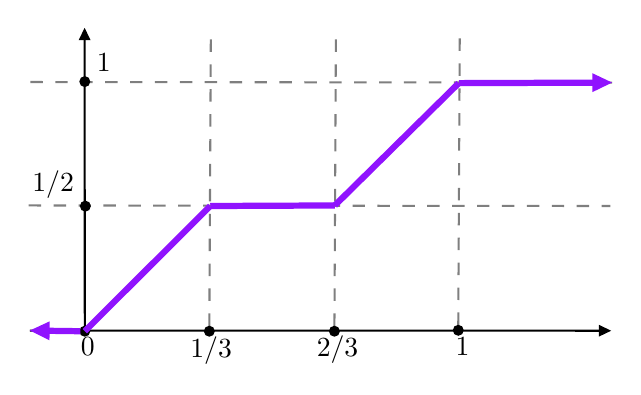
\begin{tikzpicture}[x=0.5pt,y=0.5pt,yscale=-1,xscale=1]
%uncomment if require: \path (0,300); %set diagram left start at 0, and has height of 300

%Straight Lines [id:da28165983997622934] 
\draw    (50.2,250.2) -- (467.33,250.33) ;
\draw [shift={(470.33,250.33)}, rotate = 180.02] [fill={rgb, 255:red, 0; green, 0; blue, 0 }  ][line width=0.08]  [draw opacity=0] (8.93,-4.29) -- (0,0) -- (8.93,4.29) -- cycle    ;
%Flowchart: Connector [id:dp749884860381586] 
\draw  [fill={rgb, 255:red, 0; green, 0; blue, 0 }  ,fill opacity=1 ] (86.76,250.69) .. controls (86.76,248.94) and (88.18,247.52) .. (89.93,247.52) .. controls (91.68,247.52) and (93.1,248.94) .. (93.1,250.69) .. controls (93.1,252.44) and (91.68,253.86) .. (89.93,253.86) .. controls (88.18,253.86) and (86.76,252.44) .. (86.76,250.69) -- cycle ;
%Flowchart: Connector [id:dp4945414713497278] 
\draw  [fill={rgb, 255:red, 0; green, 0; blue, 0 }  ,fill opacity=1 ] (356.67,250.02) .. controls (356.67,248.27) and (358.08,246.86) .. (359.83,246.86) .. controls (361.58,246.86) and (363,248.27) .. (363,250.02) .. controls (363,251.77) and (361.58,253.19) .. (359.83,253.19) .. controls (358.08,253.19) and (356.67,251.77) .. (356.67,250.02) -- cycle ;
%Flowchart: Connector [id:dp22339919899350247] 
\draw  [fill={rgb, 255:red, 0; green, 0; blue, 0 }  ,fill opacity=1 ] (176.76,250.69) .. controls (176.76,248.94) and (178.18,247.52) .. (179.93,247.52) .. controls (181.68,247.52) and (183.1,248.94) .. (183.1,250.69) .. controls (183.1,252.44) and (181.68,253.86) .. (179.93,253.86) .. controls (178.18,253.86) and (176.76,252.44) .. (176.76,250.69) -- cycle ;
%Flowchart: Connector [id:dp8699143961304234] 
\draw  [fill={rgb, 255:red, 0; green, 0; blue, 0 }  ,fill opacity=1 ] (267.16,250.69) .. controls (267.16,248.94) and (268.58,247.52) .. (270.33,247.52) .. controls (272.08,247.52) and (273.5,248.94) .. (273.5,250.69) .. controls (273.5,252.44) and (272.08,253.86) .. (270.33,253.86) .. controls (268.58,253.86) and (267.16,252.44) .. (267.16,250.69) -- cycle ;
%Straight Lines [id:da6785490283546702] 
\draw    (89.93,247.52) -- (89.8,34.4) ;
\draw [shift={(89.8,31.4)}, rotate = 449.97] [fill={rgb, 255:red, 0; green, 0; blue, 0 }  ][line width=0.08]  [draw opacity=0] (8.93,-4.29) -- (0,0) -- (8.93,4.29) -- cycle    ;
%Flowchart: Connector [id:dp6017519916806864] 
\draw  [fill={rgb, 255:red, 0; green, 0; blue, 0 }  ,fill opacity=1 ] (86.76,70.29) .. controls (86.76,68.54) and (88.18,67.12) .. (89.93,67.12) .. controls (91.68,67.12) and (93.1,68.54) .. (93.1,70.29) .. controls (93.1,72.04) and (91.68,73.46) .. (89.93,73.46) .. controls (88.18,73.46) and (86.76,72.04) .. (86.76,70.29) -- cycle ;
%Straight Lines [id:da7794727694597656] 
\draw [color={rgb, 255:red, 0; green, 0; blue, 0 }  ,draw opacity=0.5 ] [dash pattern={on 4.5pt off 4.5pt}]  (50.6,70.6) -- (471,71) ;
%Flowchart: Connector [id:dp9275474146310922] 
\draw  [fill={rgb, 255:red, 0; green, 0; blue, 0 }  ,fill opacity=1 ] (87.16,160.29) .. controls (87.16,158.54) and (88.58,157.12) .. (90.33,157.12) .. controls (92.08,157.12) and (93.5,158.54) .. (93.5,160.29) .. controls (93.5,162.04) and (92.08,163.46) .. (90.33,163.46) .. controls (88.58,163.46) and (87.16,162.04) .. (87.16,160.29) -- cycle ;
%Straight Lines [id:da11073911854340657] 
\draw [color={rgb, 255:red, 0; green, 0; blue, 0 }  ,draw opacity=0.5 ] [dash pattern={on 4.5pt off 4.5pt}]  (49.4,159.8) -- (469.8,160.2) ;
%Straight Lines [id:da18609205034594312] 
\draw [color={rgb, 255:red, 0; green, 0; blue, 0 }  ,draw opacity=0.5 ] [dash pattern={on 4.5pt off 4.5pt}]  (181,39.8) -- (179.93,247.52) ;
%Straight Lines [id:da06966607544396752] 
\draw [color={rgb, 255:red, 0; green, 0; blue, 0 }  ,draw opacity=0.5 ] [dash pattern={on 4.5pt off 4.5pt}]  (271.4,39.8) -- (270.33,247.52) ;
%Straight Lines [id:da20245772431088271] 
\draw [color={rgb, 255:red, 0; green, 0; blue, 0 }  ,draw opacity=0.5 ] [dash pattern={on 4.5pt off 4.5pt}]  (360.9,39.13) -- (359.83,246.86) ;
%Straight Lines [id:da606177580681843] 
\draw [color={rgb, 255:red, 144; green, 19; blue, 254 }  ,draw opacity=1 ][line width=2.25]    (180.6,160.2) -- (270.6,159.8) ;
%Straight Lines [id:da9035553151015281] 
\draw [color={rgb, 255:red, 144; green, 19; blue, 254 }  ,draw opacity=1 ][line width=2.25]    (86.76,250.69) -- (55.2,250.27) ;
\draw [shift={(50.2,250.2)}, rotate = 360.77] [fill={rgb, 255:red, 144; green, 19; blue, 254 }  ,fill opacity=1 ][line width=0.08]  [draw opacity=0] (14.29,-6.86) -- (0,0) -- (14.29,6.86) -- cycle    ;
%Straight Lines [id:da8916377477896897] 
\draw [color={rgb, 255:red, 144; green, 19; blue, 254 }  ,draw opacity=1 ][line width=2.25]    (360.2,71.4) -- (466,71.02) ;
\draw [shift={(471,71)}, rotate = 539.79] [fill={rgb, 255:red, 144; green, 19; blue, 254 }  ,fill opacity=1 ][line width=0.08]  [draw opacity=0] (14.29,-6.86) -- (0,0) -- (14.29,6.86) -- cycle    ;
%Straight Lines [id:da17503309300846714] 
\draw [color={rgb, 255:red, 144; green, 19; blue, 254 }  ,draw opacity=1 ][line width=2.25]    (89.93,250.69) -- (180.6,160.2) ;
%Straight Lines [id:da41868867930852605] 
\draw [color={rgb, 255:red, 144; green, 19; blue, 254 }  ,draw opacity=1 ][line width=2.25]    (270.6,159.8) -- (360.2,71.4) ;

% Text Node
\draw (84.8,253) node [anchor=north west][inner sep=0.75pt]   [align=left] {$\displaystyle 0$};
% Text Node
\draw (355.6,253) node [anchor=north west][inner sep=0.75pt]   [align=left] {$\displaystyle 1$};
% Text Node
\draw (164,252.4) node [anchor=north west][inner sep=0.75pt]  [font=\normalsize] [align=left] {$\displaystyle 1/3$};
% Text Node
\draw (255.33,251.73) node [anchor=north west][inner sep=0.75pt]  [font=\normalsize] [align=left] {$\displaystyle 2/3$};
% Text Node
\draw (96.4,47.6) node [anchor=north west][inner sep=0.75pt]   [align=left] {$\displaystyle 1$};
% Text Node
\draw (49.8,132.4) node [anchor=north west][inner sep=0.75pt]  [font=\normalsize] [align=left] {$\displaystyle 1/2$};


\end{tikzpicture}

        \caption{$f_1$}
    \end{subfigure}%
    \begin{subfigure}{.5\textwidth}
        \centering
        

\tikzset{every picture/.style={line width=0.75pt}} %set default line width to 0.75pt        

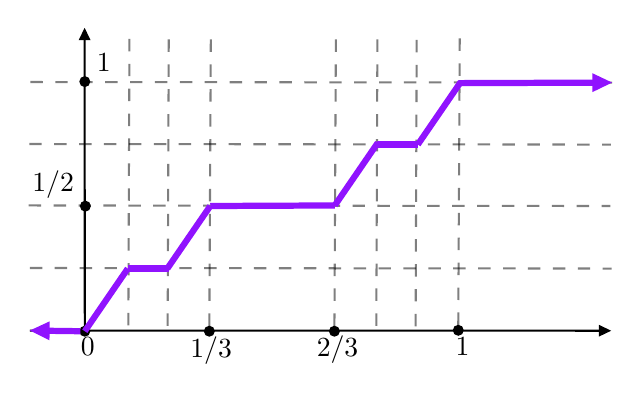
\begin{tikzpicture}[x=0.5pt,y=0.5pt,yscale=-1,xscale=1]
%uncomment if require: \path (0,300); %set diagram left start at 0, and has height of 300

%Straight Lines [id:da28165983997622934] 
\draw    (50.2,250.2) -- (467.33,250.33) ;
\draw [shift={(470.33,250.33)}, rotate = 180.02] [fill={rgb, 255:red, 0; green, 0; blue, 0 }  ][line width=0.08]  [draw opacity=0] (8.93,-4.29) -- (0,0) -- (8.93,4.29) -- cycle    ;
%Flowchart: Connector [id:dp749884860381586] 
\draw  [fill={rgb, 255:red, 0; green, 0; blue, 0 }  ,fill opacity=1 ] (86.76,250.69) .. controls (86.76,248.94) and (88.18,247.52) .. (89.93,247.52) .. controls (91.68,247.52) and (93.1,248.94) .. (93.1,250.69) .. controls (93.1,252.44) and (91.68,253.86) .. (89.93,253.86) .. controls (88.18,253.86) and (86.76,252.44) .. (86.76,250.69) -- cycle ;
%Flowchart: Connector [id:dp4945414713497278] 
\draw  [fill={rgb, 255:red, 0; green, 0; blue, 0 }  ,fill opacity=1 ] (356.67,250.02) .. controls (356.67,248.27) and (358.08,246.86) .. (359.83,246.86) .. controls (361.58,246.86) and (363,248.27) .. (363,250.02) .. controls (363,251.77) and (361.58,253.19) .. (359.83,253.19) .. controls (358.08,253.19) and (356.67,251.77) .. (356.67,250.02) -- cycle ;
%Flowchart: Connector [id:dp22339919899350247] 
\draw  [fill={rgb, 255:red, 0; green, 0; blue, 0 }  ,fill opacity=1 ] (176.76,250.69) .. controls (176.76,248.94) and (178.18,247.52) .. (179.93,247.52) .. controls (181.68,247.52) and (183.1,248.94) .. (183.1,250.69) .. controls (183.1,252.44) and (181.68,253.86) .. (179.93,253.86) .. controls (178.18,253.86) and (176.76,252.44) .. (176.76,250.69) -- cycle ;
%Flowchart: Connector [id:dp8699143961304234] 
\draw  [fill={rgb, 255:red, 0; green, 0; blue, 0 }  ,fill opacity=1 ] (267.16,250.69) .. controls (267.16,248.94) and (268.58,247.52) .. (270.33,247.52) .. controls (272.08,247.52) and (273.5,248.94) .. (273.5,250.69) .. controls (273.5,252.44) and (272.08,253.86) .. (270.33,253.86) .. controls (268.58,253.86) and (267.16,252.44) .. (267.16,250.69) -- cycle ;
%Straight Lines [id:da6785490283546702] 
\draw    (89.93,247.52) -- (89.8,34.4) ;
\draw [shift={(89.8,31.4)}, rotate = 449.97] [fill={rgb, 255:red, 0; green, 0; blue, 0 }  ][line width=0.08]  [draw opacity=0] (8.93,-4.29) -- (0,0) -- (8.93,4.29) -- cycle    ;
%Flowchart: Connector [id:dp6017519916806864] 
\draw  [fill={rgb, 255:red, 0; green, 0; blue, 0 }  ,fill opacity=1 ] (86.76,70.29) .. controls (86.76,68.54) and (88.18,67.12) .. (89.93,67.12) .. controls (91.68,67.12) and (93.1,68.54) .. (93.1,70.29) .. controls (93.1,72.04) and (91.68,73.46) .. (89.93,73.46) .. controls (88.18,73.46) and (86.76,72.04) .. (86.76,70.29) -- cycle ;
%Straight Lines [id:da7794727694597656] 
\draw [color={rgb, 255:red, 0; green, 0; blue, 0 }  ,draw opacity=0.5 ] [dash pattern={on 4.5pt off 4.5pt}]  (50.6,70.6) -- (471,71) ;
%Flowchart: Connector [id:dp9275474146310922] 
\draw  [fill={rgb, 255:red, 0; green, 0; blue, 0 }  ,fill opacity=1 ] (87.16,160.29) .. controls (87.16,158.54) and (88.58,157.12) .. (90.33,157.12) .. controls (92.08,157.12) and (93.5,158.54) .. (93.5,160.29) .. controls (93.5,162.04) and (92.08,163.46) .. (90.33,163.46) .. controls (88.58,163.46) and (87.16,162.04) .. (87.16,160.29) -- cycle ;
%Straight Lines [id:da11073911854340657] 
\draw [color={rgb, 255:red, 0; green, 0; blue, 0 }  ,draw opacity=0.5 ] [dash pattern={on 4.5pt off 4.5pt}]  (49.4,159.8) -- (469.8,160.2) ;
%Straight Lines [id:da18609205034594312] 
\draw [color={rgb, 255:red, 0; green, 0; blue, 0 }  ,draw opacity=0.5 ] [dash pattern={on 4.5pt off 4.5pt}]  (181,39.8) -- (179.93,247.52) ;
%Straight Lines [id:da06966607544396752] 
\draw [color={rgb, 255:red, 0; green, 0; blue, 0 }  ,draw opacity=0.5 ] [dash pattern={on 4.5pt off 4.5pt}]  (271.4,39.8) -- (270.33,247.52) ;
%Straight Lines [id:da20245772431088271] 
\draw [color={rgb, 255:red, 0; green, 0; blue, 0 }  ,draw opacity=0.5 ] [dash pattern={on 4.5pt off 4.5pt}]  (360.9,39.13) -- (359.83,246.86) ;
%Straight Lines [id:da606177580681843] 
\draw [color={rgb, 255:red, 144; green, 19; blue, 254 }  ,draw opacity=1 ][line width=2.25]    (180.6,160.2) -- (270.6,159.8) ;
%Straight Lines [id:da6190276976837994] 
\draw [color={rgb, 255:red, 0; green, 0; blue, 0 }  ,draw opacity=0.5 ] [dash pattern={on 4.5pt off 4.5pt}]  (301.4,39.8) -- (300.6,249.8) ;
%Straight Lines [id:da01438202404019795] 
\draw [color={rgb, 255:red, 0; green, 0; blue, 0 }  ,draw opacity=0.5 ] [dash pattern={on 4.5pt off 4.5pt}]  (329.8,40.2) -- (329,250.2) ;
%Straight Lines [id:da48628391564380014] 
\draw [color={rgb, 255:red, 0; green, 0; blue, 0 }  ,draw opacity=0.5 ] [dash pattern={on 4.5pt off 4.5pt}]  (122.2,39.4) -- (121.4,249.4) ;
%Straight Lines [id:da39031694026462715] 
\draw [color={rgb, 255:red, 0; green, 0; blue, 0 }  ,draw opacity=0.5 ] [dash pattern={on 4.5pt off 4.5pt}]  (150.6,39.8) -- (149.8,249.8) ;
%Straight Lines [id:da09573892223203795] 
\draw [color={rgb, 255:red, 0; green, 0; blue, 0 }  ,draw opacity=0.5 ] [dash pattern={on 4.5pt off 4.5pt}]  (50.2,205) -- (470.6,205.4) ;
%Straight Lines [id:da06969893090873747] 
\draw [color={rgb, 255:red, 0; green, 0; blue, 0 }  ,draw opacity=0.5 ] [dash pattern={on 4.5pt off 4.5pt}]  (49.8,115.4) -- (470.2,115.8) ;
%Straight Lines [id:da7110895807715119] 
\draw [color={rgb, 255:red, 144; green, 19; blue, 254 }  ,draw opacity=1 ][line width=2.25]    (121,205.4) -- (150.6,205.4) ;
%Straight Lines [id:da8549748831013564] 
\draw [color={rgb, 255:red, 144; green, 19; blue, 254 }  ,draw opacity=1 ][line width=2.25]    (301,115.8) -- (330.6,115.8) ;
%Straight Lines [id:da9035553151015281] 
\draw [color={rgb, 255:red, 144; green, 19; blue, 254 }  ,draw opacity=1 ][line width=2.25]    (86.76,250.69) -- (55.2,250.27) ;
\draw [shift={(50.2,250.2)}, rotate = 360.77] [fill={rgb, 255:red, 144; green, 19; blue, 254 }  ,fill opacity=1 ][line width=0.08]  [draw opacity=0] (14.29,-6.86) -- (0,0) -- (14.29,6.86) -- cycle    ;
%Straight Lines [id:da8916377477896897] 
\draw [color={rgb, 255:red, 144; green, 19; blue, 254 }  ,draw opacity=1 ][line width=2.25]    (360.2,71.4) -- (466,71.02) ;
\draw [shift={(471,71)}, rotate = 539.79] [fill={rgb, 255:red, 144; green, 19; blue, 254 }  ,fill opacity=1 ][line width=0.08]  [draw opacity=0] (14.29,-6.86) -- (0,0) -- (14.29,6.86) -- cycle    ;
%Straight Lines [id:da5648149455654867] 
\draw [color={rgb, 255:red, 144; green, 19; blue, 254 }  ,draw opacity=1 ][line width=2.25]    (89.93,250.69) -- (121,205.4) ;
%Straight Lines [id:da5935848812770368] 
\draw [color={rgb, 255:red, 144; green, 19; blue, 254 }  ,draw opacity=1 ][line width=2.25]    (149.53,205.49) -- (180.6,160.2) ;
%Straight Lines [id:da6693118537340619] 
\draw [color={rgb, 255:red, 144; green, 19; blue, 254 }  ,draw opacity=1 ][line width=2.25]    (270.6,159.8) -- (301.67,114.51) ;
%Straight Lines [id:da8194472116721105] 
\draw [color={rgb, 255:red, 144; green, 19; blue, 254 }  ,draw opacity=1 ][line width=2.25]    (330.6,115.8) -- (361.67,70.51) ;

% Text Node
\draw (84.8,253) node [anchor=north west][inner sep=0.75pt]   [align=left] {$\displaystyle 0$};
% Text Node
\draw (355.6,253) node [anchor=north west][inner sep=0.75pt]   [align=left] {$\displaystyle 1$};
% Text Node
\draw (164,252.4) node [anchor=north west][inner sep=0.75pt]  [font=\normalsize] [align=left] {$\displaystyle 1/3$};
% Text Node
\draw (255.33,251.73) node [anchor=north west][inner sep=0.75pt]  [font=\normalsize] [align=left] {$\displaystyle 2/3$};
% Text Node
\draw (96.4,47.6) node [anchor=north west][inner sep=0.75pt]   [align=left] {$\displaystyle 1$};
% Text Node
\draw (49.8,132.4) node [anchor=north west][inner sep=0.75pt]  [font=\normalsize] [align=left] {$\displaystyle 1/2$};


\end{tikzpicture}

        \caption{$f_2$}
    \end{subfigure}
    \begin{subfigure}{.5\textwidth}
        \centering
        

\tikzset{every picture/.style={line width=0.75pt}} %set default line width to 0.75pt        

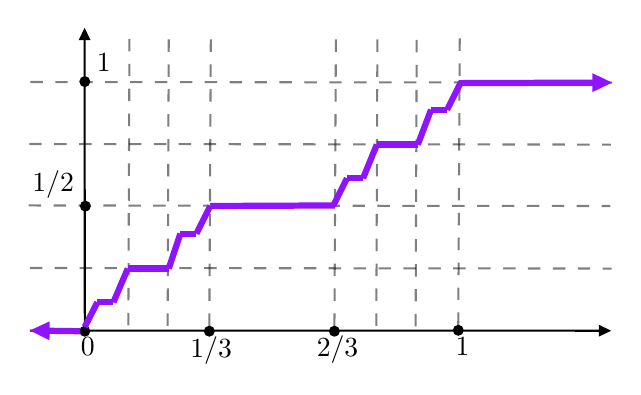
\begin{tikzpicture}[x=0.5pt,y=0.5pt,yscale=-1,xscale=1]
%uncomment if require: \path (0,300); %set diagram left start at 0, and has height of 300

%Straight Lines [id:da28165983997622934] 
\draw    (50.2,250.2) -- (467.33,250.33) ;
\draw [shift={(470.33,250.33)}, rotate = 180.02] [fill={rgb, 255:red, 0; green, 0; blue, 0 }  ][line width=0.08]  [draw opacity=0] (8.93,-4.29) -- (0,0) -- (8.93,4.29) -- cycle    ;
%Flowchart: Connector [id:dp749884860381586] 
\draw  [fill={rgb, 255:red, 0; green, 0; blue, 0 }  ,fill opacity=1 ] (86.76,250.69) .. controls (86.76,248.94) and (88.18,247.52) .. (89.93,247.52) .. controls (91.68,247.52) and (93.1,248.94) .. (93.1,250.69) .. controls (93.1,252.44) and (91.68,253.86) .. (89.93,253.86) .. controls (88.18,253.86) and (86.76,252.44) .. (86.76,250.69) -- cycle ;
%Flowchart: Connector [id:dp4945414713497278] 
\draw  [fill={rgb, 255:red, 0; green, 0; blue, 0 }  ,fill opacity=1 ] (356.67,250.02) .. controls (356.67,248.27) and (358.08,246.86) .. (359.83,246.86) .. controls (361.58,246.86) and (363,248.27) .. (363,250.02) .. controls (363,251.77) and (361.58,253.19) .. (359.83,253.19) .. controls (358.08,253.19) and (356.67,251.77) .. (356.67,250.02) -- cycle ;
%Flowchart: Connector [id:dp22339919899350247] 
\draw  [fill={rgb, 255:red, 0; green, 0; blue, 0 }  ,fill opacity=1 ] (176.76,250.69) .. controls (176.76,248.94) and (178.18,247.52) .. (179.93,247.52) .. controls (181.68,247.52) and (183.1,248.94) .. (183.1,250.69) .. controls (183.1,252.44) and (181.68,253.86) .. (179.93,253.86) .. controls (178.18,253.86) and (176.76,252.44) .. (176.76,250.69) -- cycle ;
%Flowchart: Connector [id:dp8699143961304234] 
\draw  [fill={rgb, 255:red, 0; green, 0; blue, 0 }  ,fill opacity=1 ] (267.16,250.69) .. controls (267.16,248.94) and (268.58,247.52) .. (270.33,247.52) .. controls (272.08,247.52) and (273.5,248.94) .. (273.5,250.69) .. controls (273.5,252.44) and (272.08,253.86) .. (270.33,253.86) .. controls (268.58,253.86) and (267.16,252.44) .. (267.16,250.69) -- cycle ;
%Straight Lines [id:da6785490283546702] 
\draw    (89.93,247.52) -- (89.8,34.4) ;
\draw [shift={(89.8,31.4)}, rotate = 449.97] [fill={rgb, 255:red, 0; green, 0; blue, 0 }  ][line width=0.08]  [draw opacity=0] (8.93,-4.29) -- (0,0) -- (8.93,4.29) -- cycle    ;
%Flowchart: Connector [id:dp6017519916806864] 
\draw  [fill={rgb, 255:red, 0; green, 0; blue, 0 }  ,fill opacity=1 ] (86.76,70.29) .. controls (86.76,68.54) and (88.18,67.12) .. (89.93,67.12) .. controls (91.68,67.12) and (93.1,68.54) .. (93.1,70.29) .. controls (93.1,72.04) and (91.68,73.46) .. (89.93,73.46) .. controls (88.18,73.46) and (86.76,72.04) .. (86.76,70.29) -- cycle ;
%Straight Lines [id:da7794727694597656] 
\draw [color={rgb, 255:red, 0; green, 0; blue, 0 }  ,draw opacity=0.5 ] [dash pattern={on 4.5pt off 4.5pt}]  (50.6,70.6) -- (471,71) ;
%Flowchart: Connector [id:dp9275474146310922] 
\draw  [fill={rgb, 255:red, 0; green, 0; blue, 0 }  ,fill opacity=1 ] (87.16,160.29) .. controls (87.16,158.54) and (88.58,157.12) .. (90.33,157.12) .. controls (92.08,157.12) and (93.5,158.54) .. (93.5,160.29) .. controls (93.5,162.04) and (92.08,163.46) .. (90.33,163.46) .. controls (88.58,163.46) and (87.16,162.04) .. (87.16,160.29) -- cycle ;
%Straight Lines [id:da11073911854340657] 
\draw [color={rgb, 255:red, 0; green, 0; blue, 0 }  ,draw opacity=0.5 ] [dash pattern={on 4.5pt off 4.5pt}]  (49.4,159.8) -- (469.8,160.2) ;
%Straight Lines [id:da18609205034594312] 
\draw [color={rgb, 255:red, 0; green, 0; blue, 0 }  ,draw opacity=0.5 ] [dash pattern={on 4.5pt off 4.5pt}]  (181,39.8) -- (179.93,247.52) ;
%Straight Lines [id:da06966607544396752] 
\draw [color={rgb, 255:red, 0; green, 0; blue, 0 }  ,draw opacity=0.5 ] [dash pattern={on 4.5pt off 4.5pt}]  (271.4,39.8) -- (270.33,247.52) ;
%Straight Lines [id:da20245772431088271] 
\draw [color={rgb, 255:red, 0; green, 0; blue, 0 }  ,draw opacity=0.5 ] [dash pattern={on 4.5pt off 4.5pt}]  (360.9,39.13) -- (359.83,246.86) ;
%Straight Lines [id:da606177580681843] 
\draw [color={rgb, 255:red, 144; green, 19; blue, 254 }  ,draw opacity=1 ][line width=2.25]    (180.6,160.2) -- (270.6,159.8) ;
%Straight Lines [id:da6190276976837994] 
\draw [color={rgb, 255:red, 0; green, 0; blue, 0 }  ,draw opacity=0.5 ] [dash pattern={on 4.5pt off 4.5pt}]  (301.4,39.8) -- (300.6,249.8) ;
%Straight Lines [id:da01438202404019795] 
\draw [color={rgb, 255:red, 0; green, 0; blue, 0 }  ,draw opacity=0.5 ] [dash pattern={on 4.5pt off 4.5pt}]  (329.8,40.2) -- (329,250.2) ;
%Straight Lines [id:da48628391564380014] 
\draw [color={rgb, 255:red, 0; green, 0; blue, 0 }  ,draw opacity=0.5 ] [dash pattern={on 4.5pt off 4.5pt}]  (122.2,39.4) -- (121.4,249.4) ;
%Straight Lines [id:da39031694026462715] 
\draw [color={rgb, 255:red, 0; green, 0; blue, 0 }  ,draw opacity=0.5 ] [dash pattern={on 4.5pt off 4.5pt}]  (150.6,39.8) -- (149.8,249.8) ;
%Straight Lines [id:da09573892223203795] 
\draw [color={rgb, 255:red, 0; green, 0; blue, 0 }  ,draw opacity=0.5 ] [dash pattern={on 4.5pt off 4.5pt}]  (50.2,205) -- (470.6,205.4) ;
%Straight Lines [id:da06969893090873747] 
\draw [color={rgb, 255:red, 0; green, 0; blue, 0 }  ,draw opacity=0.5 ] [dash pattern={on 4.5pt off 4.5pt}]  (49.8,115.4) -- (470.2,115.8) ;
%Straight Lines [id:da7110895807715119] 
\draw [color={rgb, 255:red, 144; green, 19; blue, 254 }  ,draw opacity=1 ][line width=2.25]    (121,205.4) -- (150.6,205.4) ;
%Straight Lines [id:da8549748831013564] 
\draw [color={rgb, 255:red, 144; green, 19; blue, 254 }  ,draw opacity=1 ][line width=2.25]    (301,115.8) -- (330.6,115.8) ;
%Straight Lines [id:da2077350927120012] 
\draw [color={rgb, 255:red, 144; green, 19; blue, 254 }  ,draw opacity=1 ][line width=2.25]    (159,180.2) -- (170.6,180.2) ;
%Straight Lines [id:da21456914664853266] 
\draw [color={rgb, 255:red, 144; green, 19; blue, 254 }  ,draw opacity=1 ][line width=2.25]    (99,229.8) -- (110.6,229.8) ;
%Straight Lines [id:da24298671555035178] 
\draw [color={rgb, 255:red, 144; green, 19; blue, 254 }  ,draw opacity=1 ][line width=2.25]    (279.4,140.2) -- (291,140.2) ;
%Straight Lines [id:da5258340451472334] 
\draw [color={rgb, 255:red, 144; green, 19; blue, 254 }  ,draw opacity=1 ][line width=2.25]    (340.2,90.6) -- (351.8,90.6) ;
%Straight Lines [id:da9035553151015281] 
\draw [color={rgb, 255:red, 144; green, 19; blue, 254 }  ,draw opacity=1 ][line width=2.25]    (86.76,250.69) -- (55.2,250.27) ;
\draw [shift={(50.2,250.2)}, rotate = 360.77] [fill={rgb, 255:red, 144; green, 19; blue, 254 }  ,fill opacity=1 ][line width=0.08]  [draw opacity=0] (14.29,-6.86) -- (0,0) -- (14.29,6.86) -- cycle    ;
%Straight Lines [id:da8916377477896897] 
\draw [color={rgb, 255:red, 144; green, 19; blue, 254 }  ,draw opacity=1 ][line width=2.25]    (360.2,71.4) -- (466,71.02) ;
\draw [shift={(471,71)}, rotate = 539.79] [fill={rgb, 255:red, 144; green, 19; blue, 254 }  ,fill opacity=1 ][line width=0.08]  [draw opacity=0] (14.29,-6.86) -- (0,0) -- (14.29,6.86) -- cycle    ;
%Straight Lines [id:da6410640073141698] 
\draw [color={rgb, 255:red, 144; green, 19; blue, 254 }  ,draw opacity=1 ][line width=2.25]    (89.93,247.52) -- (99,229.8) ;
%Straight Lines [id:da9683252500703263] 
\draw [color={rgb, 255:red, 144; green, 19; blue, 254 }  ,draw opacity=1 ][line width=2.25]    (110.6,229.8) -- (121,205.4) ;
%Straight Lines [id:da9336669722783046] 
\draw [color={rgb, 255:red, 144; green, 19; blue, 254 }  ,draw opacity=1 ][line width=2.25]    (150.6,205.4) -- (159,180.2) ;
%Straight Lines [id:da3747308648649723] 
\draw [color={rgb, 255:red, 144; green, 19; blue, 254 }  ,draw opacity=1 ][line width=2.25]    (170.6,180.2) -- (180.6,160.2) ;
%Straight Lines [id:da897767378011493] 
\draw [color={rgb, 255:red, 144; green, 19; blue, 254 }  ,draw opacity=1 ][line width=2.25]    (269.4,160.2) -- (279.4,140.2) ;
%Straight Lines [id:da44587661962793557] 
\draw [color={rgb, 255:red, 144; green, 19; blue, 254 }  ,draw opacity=1 ][line width=2.25]    (291,140.2) -- (301,115.8) ;
%Straight Lines [id:da7331983887111697] 
\draw [color={rgb, 255:red, 144; green, 19; blue, 254 }  ,draw opacity=1 ][line width=2.25]    (330.6,115.8) -- (340.2,90.6) ;
%Straight Lines [id:da9029004294454352] 
\draw [color={rgb, 255:red, 144; green, 19; blue, 254 }  ,draw opacity=1 ][line width=2.25]    (351.8,90.6) -- (361.8,70.6) ;

% Text Node
\draw (84.8,253) node [anchor=north west][inner sep=0.75pt]   [align=left] {$\displaystyle 0$};
% Text Node
\draw (355.6,253) node [anchor=north west][inner sep=0.75pt]   [align=left] {$\displaystyle 1$};
% Text Node
\draw (164,252.4) node [anchor=north west][inner sep=0.75pt]  [font=\normalsize] [align=left] {$\displaystyle 1/3$};
% Text Node
\draw (255.33,251.73) node [anchor=north west][inner sep=0.75pt]  [font=\normalsize] [align=left] {$\displaystyle 2/3$};
% Text Node
\draw (96.4,47.6) node [anchor=north west][inner sep=0.75pt]   [align=left] {$\displaystyle 1$};
% Text Node
\draw (49.8,132.4) node [anchor=north west][inner sep=0.75pt]  [font=\normalsize] [align=left] {$\displaystyle 1/2$};


\end{tikzpicture}

        \caption{$f_3$}
    \end{subfigure}
    \caption{Первые три функции последовательности $\{f_n\}$.}
    \label{fig:k123}
\end{figure}

Взяв $f$ в качестве $F$ в прошлом разделе получим меру $\mu$ такую, что $\mu(C)=1$, а $\mu(\R\setminus C)=0$, где $C$~--- множество Кантора. 
Множество Кантора определяется как $C=\bigcap\limits_{n=1}^{\infty}C_n$, где 
\begin{align*}
    C_1 &= [0,\, 1]\setminus (1/3,\, 2/3)\\
    C_2 &= C_1\setminus ((1/9,\, 2/9)\cup (7/9,\, 8/9)\\
    \ldots
\end{align*}
то есть, такие множества, из которых итеративно выкидывают <<плоские>> участки функции Кантора.

\subsection{Множество неизмеримое по Лебегу.}

Вспомним понятия, связанные с мерой Лебега. Пусть $m$~--- клеточная мера: $m:\ K_d\to[0,\,+\infty]$. Далее рассматривалось ее продолжение: внешняя мера $m^*$.
И мера Лебега: $\lambda:\ \CA_{m^*}\to[0,\, +\infty]$ такая, что $\lambda(A)=m^*(A)$ (то есть сужение внешней меры на семейство всех аддитивных относительно внешней меры Лебега множеств).
$\CA_{m^*}$~--- семейство всех измеримых по Лебегу множеств. Договоримся, что $\CA_{m^*}=\mathfrak{m}_d$.
Можно написать цепочку вложений: 
\[
    K_d\subset\sigma(K_d)=\CB(\R^d)\subset \mathfrak{m}_d\subset \CP(\R^d). 
\]

Покажем, что $\mathfrak{m}_d\subsetneq \CP(\R^d)$. Построим классы эквивалентности: $x,\, y$ лежат в одном классе, если $x-y\in\Q$.
Легко проверить, что это действительно отношение эквивалентности: 
\begin{enumerate}
    \item $x\sim x$;
    \item Если $x\sim y$ и $y\sim z$, то $x\sim z$, так как $x-z=(x-y)+(y-z)\in\Q$.
\end{enumerate}
Пусть теперь $E_x=\{y\in[0,\, 1]\ \mid\ x\sim y\}$.
\begin{claim}[Аксиома выбора]
    Для любого множества $X$ существует функция $v:\ \CP(X)\to X$ такая, что $\forall A\subset X,\, A\neq\varnothing$ имеем $v(A)\in A$.
\end{claim}

Использую аксиому построим \mdef{множество Витали}:
\[
    V:=\{v(E_x):\ x\in[0,\, 1]\}.    
\]

\begin{remark}
    Если $t,\, s\in \Q$ и $t\neq s$, тогда $(V+s)\cap (V+t)=\varnothing$.

    \begin{proof}

        В самом деле, предположим противное, то есть $\exists x,\, y:\ v(E_x)+x=v(E_y)+t$. Тогда 
        \[
            v(E_y)-v(E_x)=s-t\in\Q\Rightarrow E_x=E_y\Rightarrow v(E_x)=v(E_y)\Rightarrow s=t\text{~--- противоречие.}
        \]
    \end{proof}
\end{remark}

\begin{claim}
    $V$~--- неизмеримо по Лебегу.
    
    \begin{proof}
        
        Предположим противное: $V$~--- измеримо по Лебегу. Если $\lambda(V)=0$, то $\lambda([0,\, 1])=0$, так как 
        \[
            [0,\, 1]\subset \bigcap\limits_{t\in\Q}(V+t)\Rightarrow\lambda([0,\, 1])\leqslant\sum_{t\in\Q}\underbrace{\lambda(V+t)}_{=\lambda(V)=0}.
        \]
        Поэтому $\lambda(V)>0$. Но тогда 
        \[
            \lambda([0,\, 2])\geqslant\lambda\left(\bigsqcup_{t\in[0,\, 1]\cap \Q} (V+t)\right)=
            \sum_{t\in[0,\, 1]\cap \Q}\underbrace{\lambda(V+t)}_{\lambda(V)}=+\infty\text{~--- противоречие.}
        \]

    \end{proof}
\end{claim}